\documentclass[11pt, fleqn]{article}
\usepackage{multicol}

%\usepackage[a4, frame, center, noinfo]{crop}


%You should edit DSLecture.tex, not this file!
\usepackage{amsthm}
\usepackage{latexsym}
\usepackage{amssymb}
\usepackage{verbatim}
\usepackage{enumitem,amsmath,array}
\usepackage{tikz}
\usepackage{tkz-graph}
\usepackage{bookmark}
\usetikzlibrary{positioning,chains,fit,shapes,calc}
%a4paper, margin=0.7in     , paperwidth=16cm,paperheight=24cm
%\usepackage[paperwidth=20cm,paperheight=29cm]{geometry}
\usepackage[a4paper, margin=0.7in]{geometry}
\usepackage{listings}
\usepackage{clrscode3e}
\usepackage{hyperref}
\hypersetup{
	colorlinks=true,
	linkcolor=blue,
	filecolor=magenta,      
	urlcolor=cyan,
}
\usepackage{xepersian}
%\usepackage[fontsloadable]{xepersian}

\settextfont{HM XNiloofar}
%\setdigitfont{HM XNiloofar}
%\setdigitfont{ParsiDigits}
\defpersianfont\outline[Scale=1]{HM XNiloofar Outline}

\setlength{\parindent}{1.5em}
\setlength{\parskip}{0.9em}
\renewcommand{\baselinestretch}{1.4}


\newcommand{\lecture}[3]{
%\pagestyle{empty}
{
	\begin{center}
			\vspace{-1cm}
		   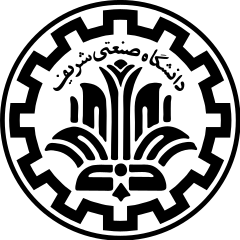
\includegraphics[scale=0.35]{Sharif}%\hfill \\[1em]  
	\end{center}
	\vspace{-8mm}

%\bf

%\begin{outline} 

%\end{outline} 

}\vspace*{-1em}
\noindent
 #2 \hfill 
\vspace{-4mm}
\rule{\textwidth}{1pt}
\ \\
}

% example environment
\newenvironment{example}
{\smallskip \noindent \emph{مثال:}}
{\hfill $\boxtimes$ \smallskip}


\newtheorem{theorem}{قضیه}
\newtheorem{proposition}{گزاره}
\newtheorem{claim}{ادعا}
\newtheorem{lemma}{لم}
\newtheorem{corollary}{نتیجه}
\newtheorem{definition}{تعریف} % Use this for non-trivial definitions.
\newcommand*{\newtitle}[1]{
\begin{large}
\textbf{#1}
\end{large}
}
\newcommand*{\newhline}{
\vspace{-7mm}
\rule{\textwidth}{1pt}

}
\newcommand*{\newsline}{
\vspace{-7mm}
\rule{8cm}{1pt}

}
\newcommand*{\maintitle}[1]{
\begin{center}
\textbf{
\LARGE{#1}
}
\end{center}
}
\usepackage{mathtools, nccmath}
\usepackage{tikz}
\usepackage{mathtools}
\usepackage{graphicx}
\usepackage{tikz} % To generate the plot from csv
\usepackage{pgfplots}
\pgfplotsset{compat=1.5}
\usetikzlibrary{patterns}
\usepackage{amssymb}% http://ctan.org/pkg/amssymb
\usepackage{pifont}% http://ctan.org/pkg/pifont
\usepackage{graphicx}

\usepackage{pgf}
\usepackage{pgfpages}
\usepackage{booktabs}



\begin{document}

\renewcommand\refname{}




\begin{center}

			\vspace{-1cm}
		   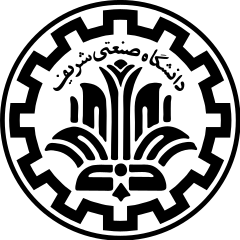
\includegraphics[scale=0.5]{Sharif}%\hfill \\[1em]  
		   \vspace{2cm}

\textbf{
\Huge{
استفاده از روش‌های مولتی مدال برای تشخیص احساس
}}
\vspace{3cm}

\textbf{
\huge{
پردازش زبان‌ها طبیعی
}}

\vspace{10mm}


\Large{
ساحل مس فروش
سروش تابش
درنا دهقانی
امین کشیری
فاطمه توحیدیان
سید علیرضا موسوی زاده
}

\vspace{4cm}

\large{
بهار ۱۴۰۱
}
\end{center}


\newpage
\section*{چکیده}



\newhline

خلاصه ی متن
 
\newhline



\begin{multicols}{2}

\section{مقدمه}


مقدمه چینی


\section{داده ها}


داده های استفاده شده

% \end{multicols}


% \begin{multicols}{2}

\section{مدل‌}


مدل استفاده شده

\section{نتایج}

نتایج پروژه


\section{نتیجه‌گیری}
نتیجه گیری


\end{multicols}


\section{منابع}



\newhline



\begin{latin}
    \begin{thebibliography}{99}
    
    \bibitem{s1}
    Inyong Shin, 2012, Income inequality and economic growth, Economic Modelling, vol. 29, no. 5, pp. 2049-2057

    \bibitem{s2}
    Pak Hung Mo, 2003, Income inequality and economic growth, Kyklos, vol. 53, no. 3, pp. 293-315

    \bibitem{s3}
    Kholeka M.  Sin-Yu H., 2021, Literature review on income inequality and economic growth, MethodsX, vol. 8, pp. 101402

    % \bibitem{}
    
    % \bibitem{s2}
    %   Statistical Centre of Iran. \url{http://Amar.org.ir}
    
    \bibitem{worldbank}
    World Bank Data. \url{http://data.worldbank.ir}
    
    % \bibitem{main}
    % Estimation of the Solow-Cobb-Douglas economic growth model with a
    % Kalman filter: An observability-based approach. \url{https://europepmc.org/backend/ptpmcrender.fcgi?accid=PMC6595187&blobtype=pdf}
    \end{thebibliography}
\end{latin}

% \bibliography{refs}

\end{document}